\documentclass{article} % For LaTeX2e
\usepackage{nips14submit_e,times}
\usepackage{hyperref}
\usepackage{url}
%\documentstyle[nips14submit_09,times,art10]{article} % For LaTeX 2.09
\usepackage{graphicx}

\title{MLCLASS\_FDU Report for CSCI567 Project}


\author{
Junming Chen
\And
Zekun Li \\
Affiliation \\
Address \\
\texttt{email} \\
\AND
Junfeng Wu \\
Affiliation \\
Address \\
\texttt{email}
}

% The \author macro works with any number of authors. There are two commands
% used to separate the names and addresses of multiple authors: \And and \AND.
%
% Using \And between authors leaves it to \LaTeX{} to determine where to break
% the lines. Using \AND forces a linebreak at that point. So, if \LaTeX{}
% puts 3 of 4 authors names on the first line, and the last on the second
% line, try using \AND instead of \And before the third author name.

\newcommand{\fix}{\marginpar{FIX}}
\newcommand{\new}{\marginpar{NEW}}

%\nipsfinalcopy % Uncomment for camera-ready version
\nipsfinalcopy
\begin{document}


\maketitle

\begin{abstract}
This is a project using Random Forest Algorithm to predict hourly rainfall. After data preprocessing, the optimization is mostly done by feature transformation and selection. The final result reached 23.75398 variance and rank 51 of all teams.
\end{abstract}

\section{Data Processing}

\subsection{Overview}
First of all, there are about 38\% totally missing data in the data set and many data entries with incomplete data. As the MAE changing of this competition, we only predict one target value for each ID's data and process those data with at least one of the Ref values is non-null.

\subsection{Preprocessing}

For the data preprocessing, the first rule is to extract only valid data entries, which has at least one of the Ref values is non-null. Then according to common sense, we eliminate the reflectivity values, composite values and reference values which are below zero. \\
\\
It is also essential to eliminate abnormal data and some outliers. We firstly eliminate the negative values in features Ref, RefComposite because they should be positive. From the expected rain frequency histogram, we found out that, most values are lower than 100. However, there are some extremely large values more than 1,000 and should be eliminate. We choose the threshold of 70 at last because the bucket element droped to only 300 from bucket (68,70) while all the bucket in range (0,68) with interval of 2 have more than 2,000 data entries fall into them.\\

\begin{figure}[h]
\fbox{\rule[-.5cm]{0cm}{4cm}
\begin{minipage}[t]{0.5\linewidth}
\centering
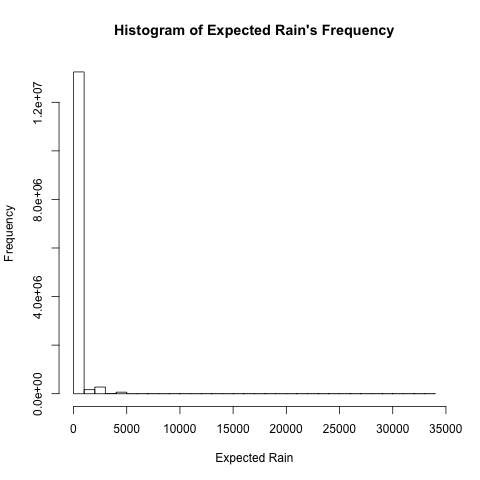
\includegraphics[width=2.5in]{distribution}
\label{fig:side:a}
\end{minipage}%
\begin{minipage}[t]{0.5\linewidth}
\centering
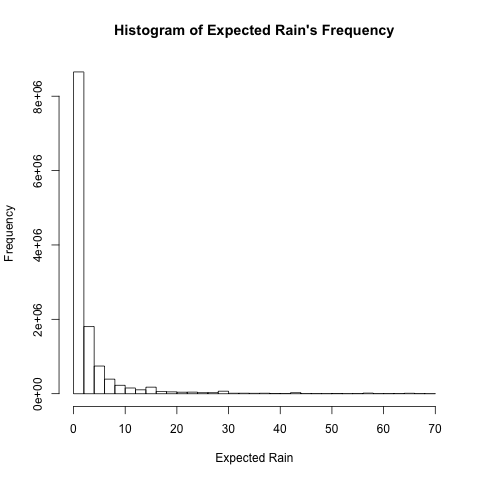
\includegraphics[width=2.5in]{distribution-70}
\label{fig:side:b}
\end{minipage}
 \rule[-.5cm]{0cm}{0cm}}
\caption{Density scatter of relation between Ref, RefComp50, Ref50 and Expect Rain}
\end{figure}




\section{Feature Selection}
\subsection{Basic matrice}
From the official data description, we have to generate only one line of feature value for each given data group by ID. Thus, we firstly transfer the given data using mean, variance or summation.\\
\\
We first plot some density graph and saw that the mean value of Ref seems correlated with expected value. The variance of Ref is different from mean but we can see from the plot that most variance is relatively low with expected value lower than 2. Thus, using these features could be helpful for the prediction.\\
\\
Some basic features we selected:
\begin{itemize}
\item\textbf{Ref}: Using mean, variance and summation of Ref group by ID.
\item\textbf{Ref\_5x5, RefComposite and RefComposite\_5x5}: Using both mean and variance of each feature group by ID.
\item\textbf{rhoHV, RhoHV\_5x5, Zdr and Zdr\_5x5}: Using only mean of each feature group by ID.
\item\textbf{rhoHV, RhoHV\_5x5, Zdr and Zdr\_5x5}: Using only mean of each feature group by ID.
\item\textbf{Kdp}: Using only mean of each feature group by ID. This didn't work well so not used in final features.
\item\textbf{Number of records}: Using the record number in an ID group as a feature.
\item\textbf{Number of Ref's missing values}: Using the number of Ref's missing value in an ID group as a feature.
\end{itemize}

\begin{figure}[h]
\fbox{\rule[-.5cm]{0cm}{4cm}
\begin{minipage}[t]{0.33\linewidth}
\centering
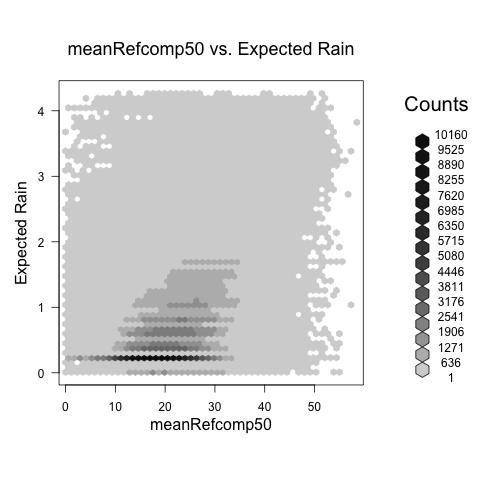
\includegraphics[width=1.8in]{feature1}
\label{fig:side:a}
\end{minipage}%
\begin{minipage}[t]{0.33\linewidth}
\centering
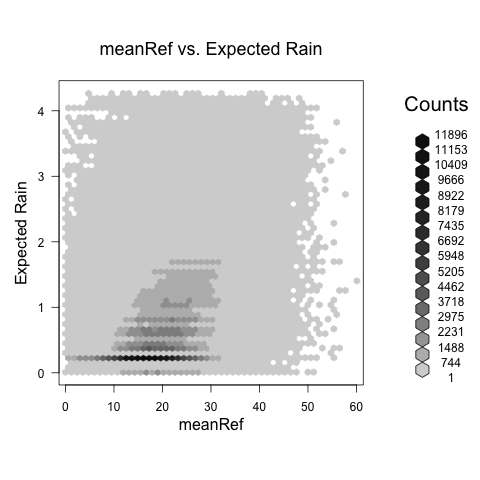
\includegraphics[width=1.8in]{feature6}
\label{fig:side:b}
\end{minipage}
\begin{minipage}[t]{0.33\linewidth}
\centering
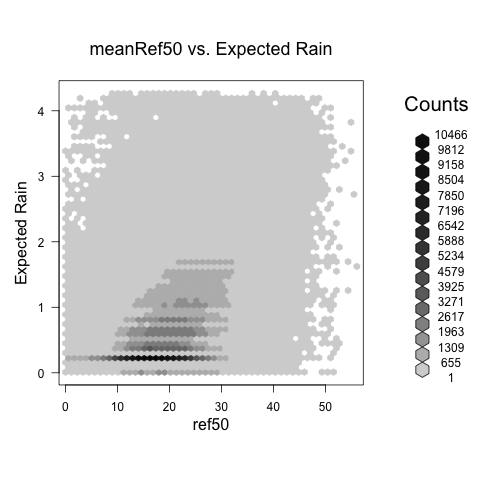
\includegraphics[width=1.8in]{feature2}
\label{fig:side:c}
\end{minipage}
 \rule[-.5cm]{0cm}{0cm}}
\caption{Density scatter of relation between mean Ref, RefComp50, Ref50 and Expect Rain}
\end{figure}


\begin{figure}[h]
\fbox{\rule[-.5cm]{0cm}{4cm}
\begin{minipage}[t]{0.33\linewidth}
\centering
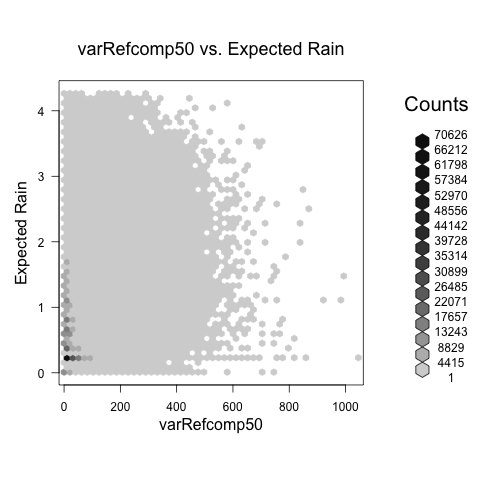
\includegraphics[width=1.8in]{feature4}
\label{fig:side:a}
\end{minipage}%
\begin{minipage}[t]{0.33\linewidth}
\centering
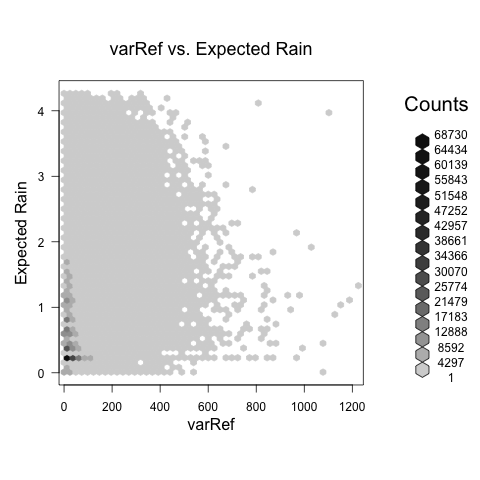
\includegraphics[width=1.8in]{feature3}
\label{fig:side:b}
\end{minipage}
\begin{minipage}[t]{0.33\linewidth}
\centering
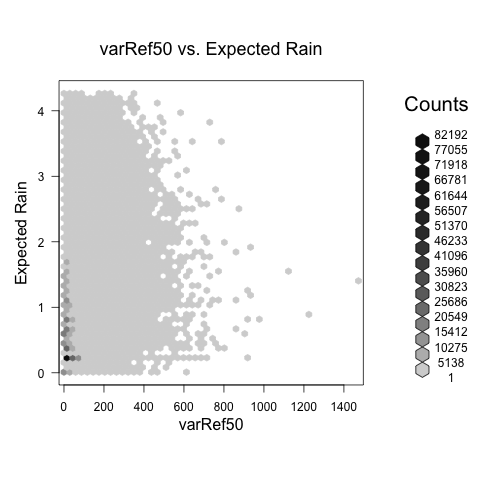
\includegraphics[width=1.8in]{feature5}
\label{fig:side:c}
\end{minipage}
 \rule[-.5cm]{0cm}{0cm}}
\caption{Density scatter of relation between variance Ref, RefComp50, Ref50 and Expect Rain}
\end{figure}

\subsection{New Features}
\textbf{Combining Marshall-Palmer Observation}: From the official description, Marshall-Palmer relationship is a method to predict the gauge observation using radar data. It used the Ref data combined with minutes\_past to calculate the prediction and it is a reasonable way to take minutes\_past into account.\\
\\We simply add the  Marshall-Palmer observation into the training feature, but it will lower the prediction accuracy so not used in final features.\\\\

\textbf{Combining transferred KDP}: Because the former combination failed, we sought another way to do numeric calculation of predicted raining rate. We found a new formula which can also do this. 
\begin{equation} 
rate = \sum((sign(Kdp)*(kdpzdr\_aa)*(|Kdp|^{kdpzdr\_bb})(ZDR ^ {kdpzdr\_cc}))
\end{equation}
where $kdpzdr\_aa = 136, kdpzdr\_bb = 0.968, kdpzdr\_cc = -2.86$.\\\\
We added the  raining rate predicted by KDP into the training feature, but it will lower the prediction accuracy so not used in final features.\\
\\
\textbf{Combining radardist\_km}: Because radar usually cover a certain area which is related to the radardist\_km. Then we examined new features of original Ref and RefComposite divided by radardist\_km, and original Ref and RefComposite divided by radardist\_km$^2$.\\
\\The second new feature using radardist\_km$^2$ seems more reasonable because if the cover area of the radar is a circle, the area is related to radardist\_km$^2$. However, the cross validation result showed that the first new feature works better, so we only added original Ref and RefComposite divided by radardist\_km as for final features.

\textbf{Combining difference on Ref between two consecutive time}: Because we haven't got used of time, we tried to add features of averaged Ref and RefComposite difference between two consecutive record in same ID. The seemingly more reasonable feature is to add a feature which is the consecutive Ref and RefComposite difference divided by time difference. However, It worked worse than the former one. So only averaged Ref and RefComposite difference was added into the final features.

\subsection{Final Features}
We do the feature selection process and only add a feature when adding it can improve the cross validation's mean squared error. Finally 40 features are selected and can be categorized as:
\begin{itemize}
\item\textbf{Ref(including all percentile data)}: Using mean, variance and summation.
\item\textbf{RefComposite(including all percentile data)}: Using mean, variance.
\item\textbf{rhoHV and zdr(including all percentile data)}: Using mean.
\item\textbf{mean Ref and RefComposite divide radardist\_km}: Using value of this equation.
\item\textbf{difference on Ref and RefComposite between two consecutive time}: Using value of this equation.
\end{itemize}

\section{Algorithm}

Our first attempt is using Random Forest Algorithm. The reason is:
\begin{itemize}
\item It is good classifier for most data and scenes.
\item It can handle large amount of variables.
\item It gives features different importance.
\item It can work even with high percentage missing data.
\item The speed is relatively fast.
\end{itemize}

\section{Evaluation}


\subsection{Evaluation on Feature Selections}

We implement the Random Forest regression based on the starter script in Kaggle Forum. In the starter script, the selected features are:

\begin{itemize}
\item mean and sum of Ref
\item mean of Refcomp
\item Distance
\item Number of records and missing values
\end{itemize}

Table \ref{feat-cmp-table} shows the improvement after adding the features we selected. And Table \ref{feat-importance} shows the importance among all the selected features

\begin{table}[h]
\caption{Feature Selection Evaluation}
\label{feat-cmp-table}
\begin{center}
\begin{tabular}{ll}
\multicolumn{1}{c}{}  &\multicolumn{1}{c}{\bf MAE}
\\ \hline \\
Random Froest in starter script             &23.89669 \\
Random Froest after adding features             &23.75398 \\
\end{tabular}
\end{center}
\end{table}

\begin{table}[h]
\caption{Variable Importances}
\label{feat-importance}
\begin{center}
\begin{tabular}{llll}
\multicolumn{1}{c}{\bf Order}  &\multicolumn{1}{c}{\bf Variable}  &\multicolumn{1}{c}{\bf Scaled Importance} &\multicolumn{1}{c}{\bf Percentage}
\\ \hline \\
1 &mean of Ref\_5x5\_90th  &1.000000   &0.148810  \\
2 &mean of Ref\_5x5\_50th  &0.631968   &0.094043  \\
3 &mean of RefComposite\_5x5\_90th  &0.501650   &0.074651  \\
4 &mean of Ref  &0.421761   &0.062762  \\
5 &Radardist\_km  &0.281814  &0.041937  \\
\ldots\\
41 &max of Kdp  &0.063436   &0.009042\\
42 &mean of RhoHV\_5x5\_90th  &0.062761  &0.008945\\
43 &min of Kdp  &0.062702   &0.008937\\
44 &mean of RhoHV\_5x5\_10th  &0.059808   &0.008524\\
45 &mean of RhoHV\_5x5\_50th  &0.059564   &0.008490\\
\end{tabular}
\end{center}
\end{table}


\subsection{Evaluation on Different Regression Method}

\begin{table}[h]
\caption{Feature Selection Evaluation}
\label{model-cmp-table}
\begin{center}
\begin{tabular}{ll}
\multicolumn{1}{c}{\bf Model}  &\multicolumn{1}{c}{\bf MAE}
\\ \hline \\
xxx             &23.79669 \\
Random Froest            &23.75398 \\
\end{tabular}
\end{center}
\end{table}

\subsubsection*{References}

References follow the acknowledgments. Use unnumbered third level heading for
the references. Any choice of citation style is acceptable as long as you are
consistent. It is permissible to reduce the font size to `small' (9-point) 
when listing the references. {\bf Remember that this year you can use
a ninth page as long as it contains \emph{only} cited references.}

\small{
[1] https://www.eol.ucar.edu/projects/dynamo/spol/parameters/rain\_rate/rain\_rates.html

[2] http://glossary.ametsoc.org/wiki/Marshall-palmer\_relation
}
\end{document}